\section{Introduction}

With our simple expressions for the reservation price and quote
spread derived from our approximations, and the intuitive procedure
described at the end of section \ref{sec:3.8}, we can easily test 
the performance of our strategy using numerical simulation. We use the Python 
programming language along with some third party but standard packages such as 
numpy and matplotlib to implement our code, record our results and produce the 
plots seen in this section. 

In what follows, we will replicate the results obtained 
by \textcite{AS2008}, comparing and contrasting the results of the ``inventory'' strategy
we derived in chapter \ref{chap:3} to those of a ``symmetric'' strategy that simply
quotes the average spread of the inventory strategy at all times regardless of current
inventory. 

The conclusions drawn from our results are much the same as those drawn 
from the results presented by Avellaneda and Stoikov, seeing as we replicate their 
results quite closely. However, they do not provide the code behind their numerical 
simulations, so it is not possible to know if our methodology is exactly the same as 
theirs. Our contribution to the literature then, for this chapter, is to provide in 
full the Python code behind our results, which can be found in appendix \ref{app:B}.

\section{Numerical Simulations - Avellaneda \& Stoikov}

\begin{figure}[ht!]
    \centering
        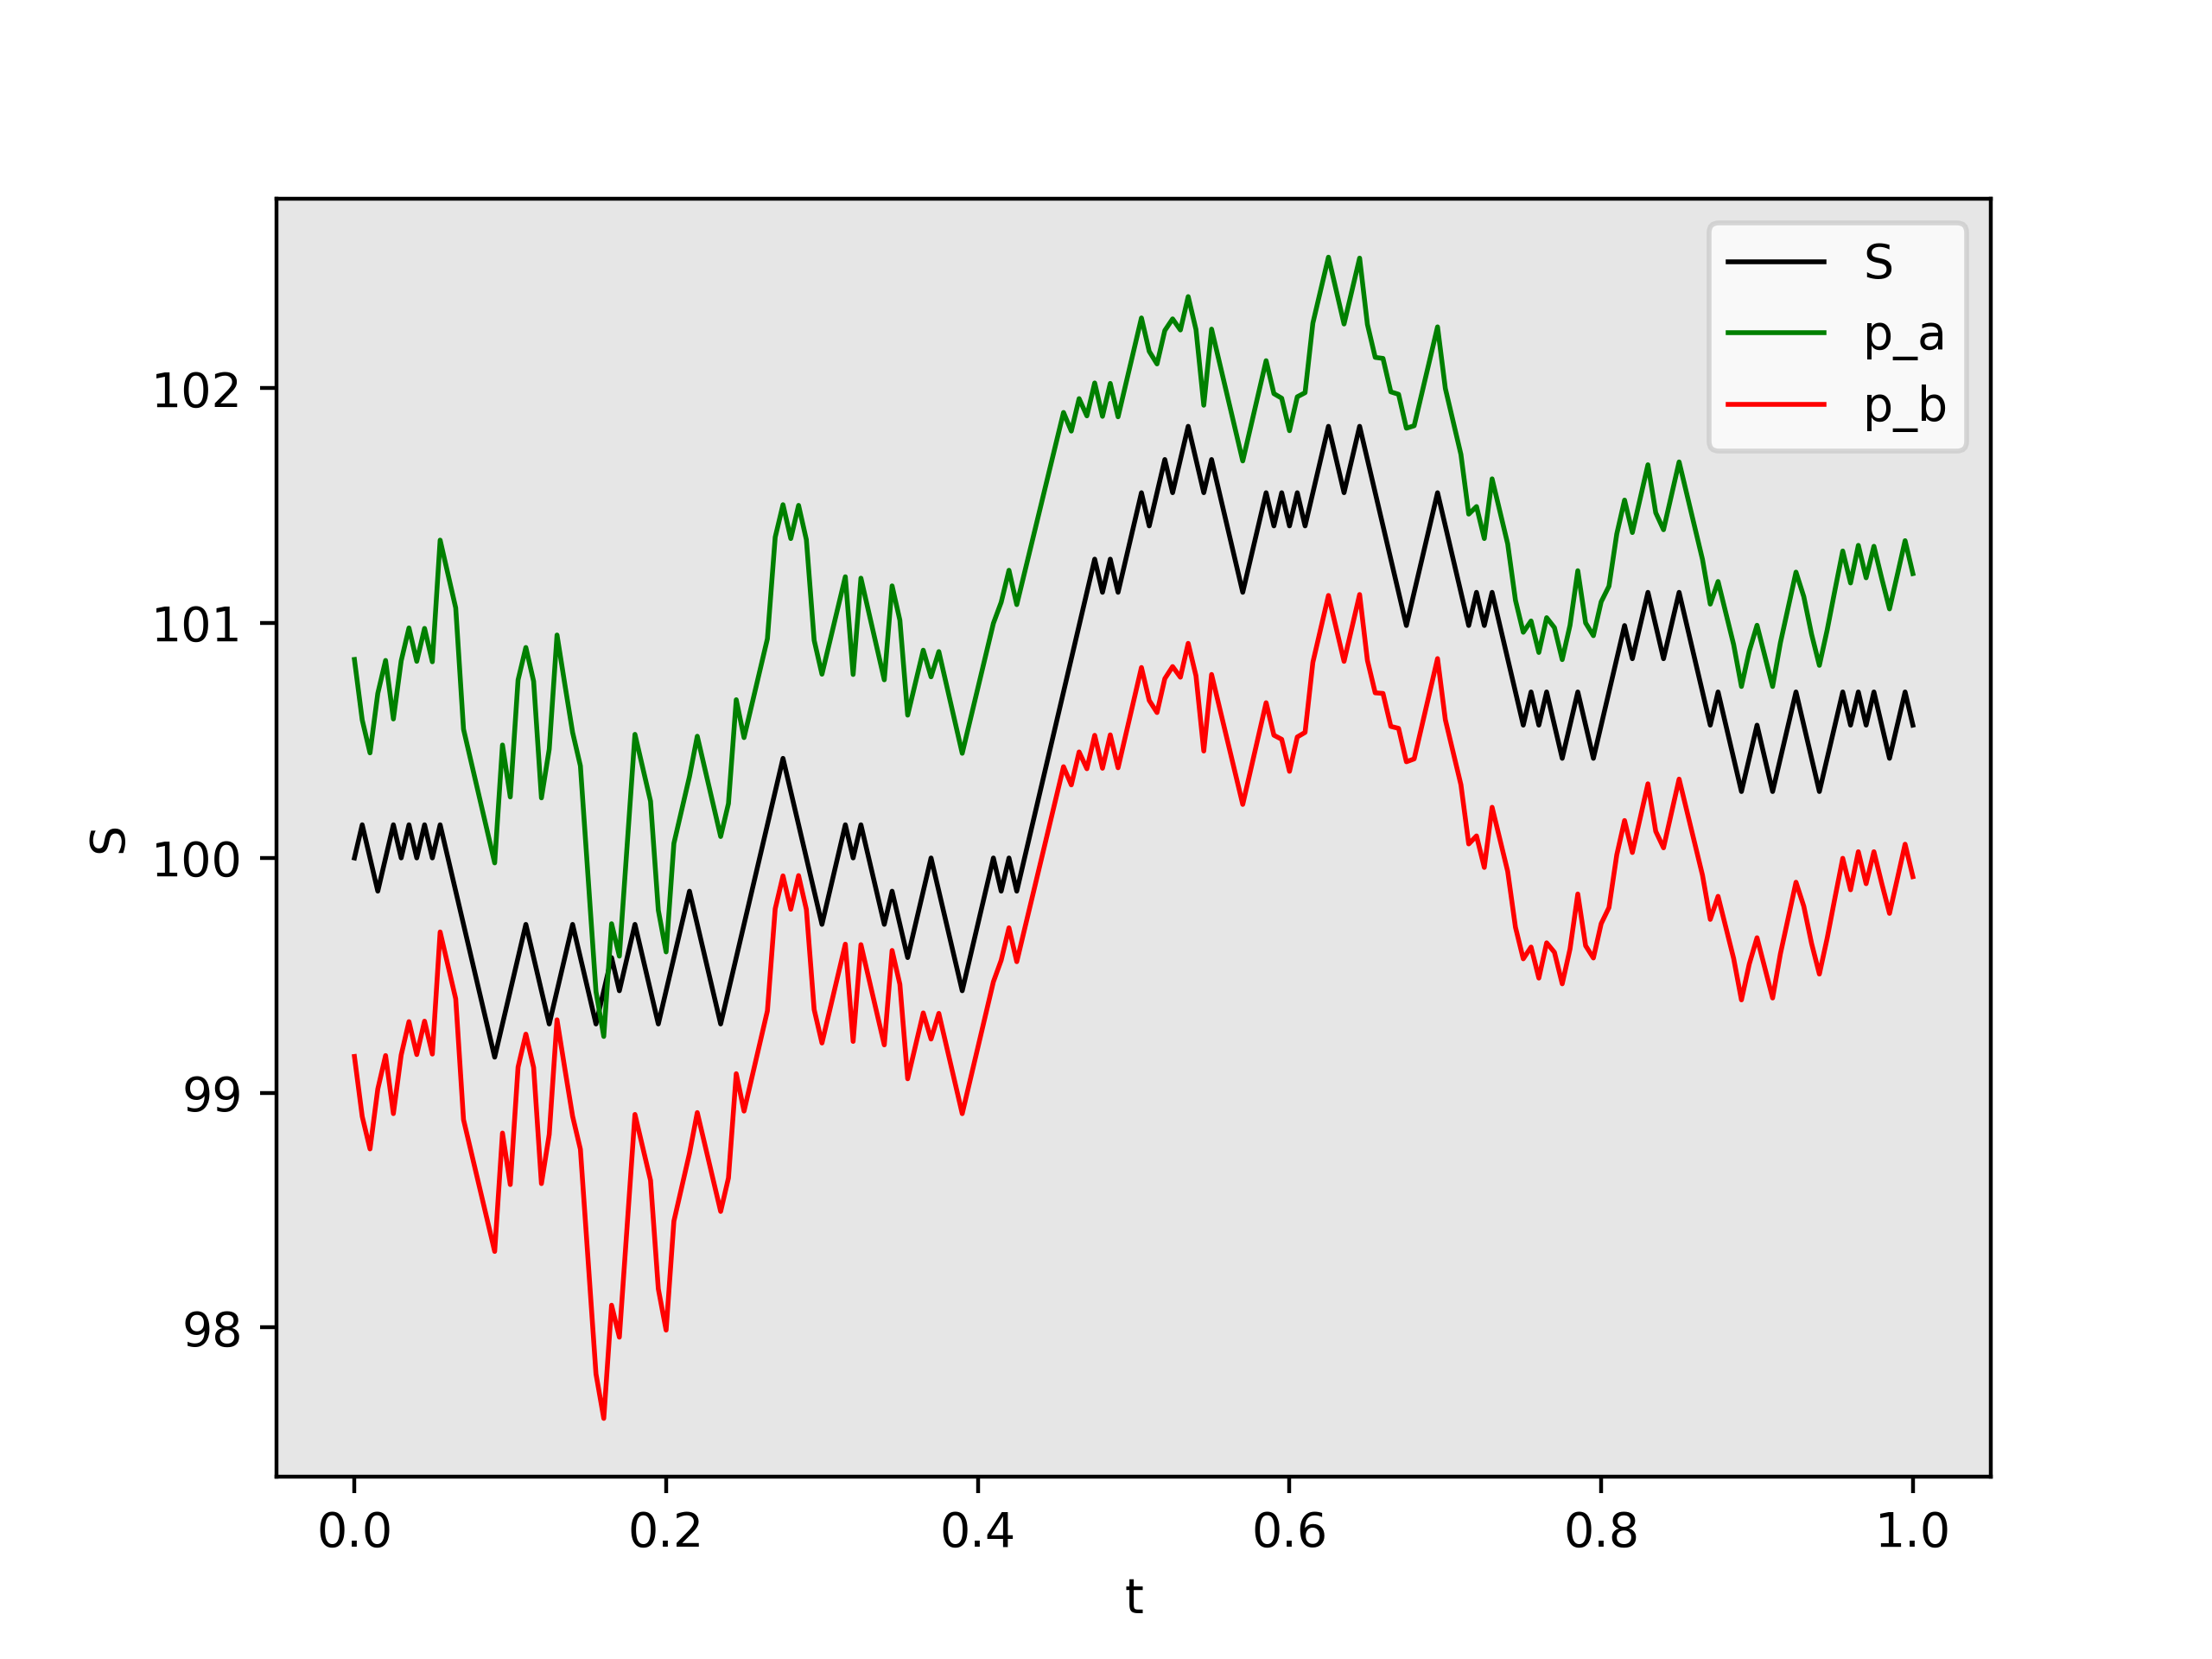
\includegraphics[width=0.75\linewidth]{sample-path.png}
        \caption{Sample path for $\gamma=0.1$}
        \label{fig:sample-paths}
\end{figure}

In figures \ref{fig:sample-paths}, \ref{fig:inventory} and \ref{fig:pnl}, we can see 
plotted the evolution of the mid-price and our agent's bid and ask quotes, inventory,
cash flow and total portfolio value over time as incoming market-orders are sampled.

We can identify the effect of varying levels of inventory on our bid 
and ask quotes as we first discussed all the way back in chapter \ref{chap:1}: at 
$t\approx0.3$ for example, the agent was short stock and hence set her quotes around 
a high reservation price, resulting in a bid price that almost coincided with the 
midprice. Conversely, at $t\approx0.2$, the agent was long stock, setting her quotes 
around a low reservation price. We can also see the effect of time - as we reach $T$, 
the quotes become more and more symmetric as the agent become more and more certain 
about the terminal price $S_T$.

In figure \ref{fig:results-gamma01} we present the results and PnL 
distributions for 10000 simulations with $\gamma=0.1$. We obtain 
an identical mean spread to \textcite{AS2008}, which is to be expected
as the calculation for the mean spread does not depend on either 
the sampling of the mid-price nor the sampling of market orders.
All of our results for the mean and standard deviation of the profit
and final inventory are within $0.1$ of those presented in the original
paper, with the exception of the standard deviation of final inventory 
where my figure of 13.1 is 0.4 above the 12.7 reported by Avellaneda
and Stoikov.

The higher mean and larger variance of profits for the symmetric strategy is clearly
visible in the PnL distribution. This can be explained by the fact that the symmetric 
strategy on average receives more orders than the inventory strategy as it tends 
to quote a tighter spread throughout the trading session, however, it also accumulates
higher inventories and so the profits of the strategy are driven much more by the
position accumulated in the asset than by the cash flow accumulated from the bid-ask
spread.

\begin{figure}[ht!]
    \centering
    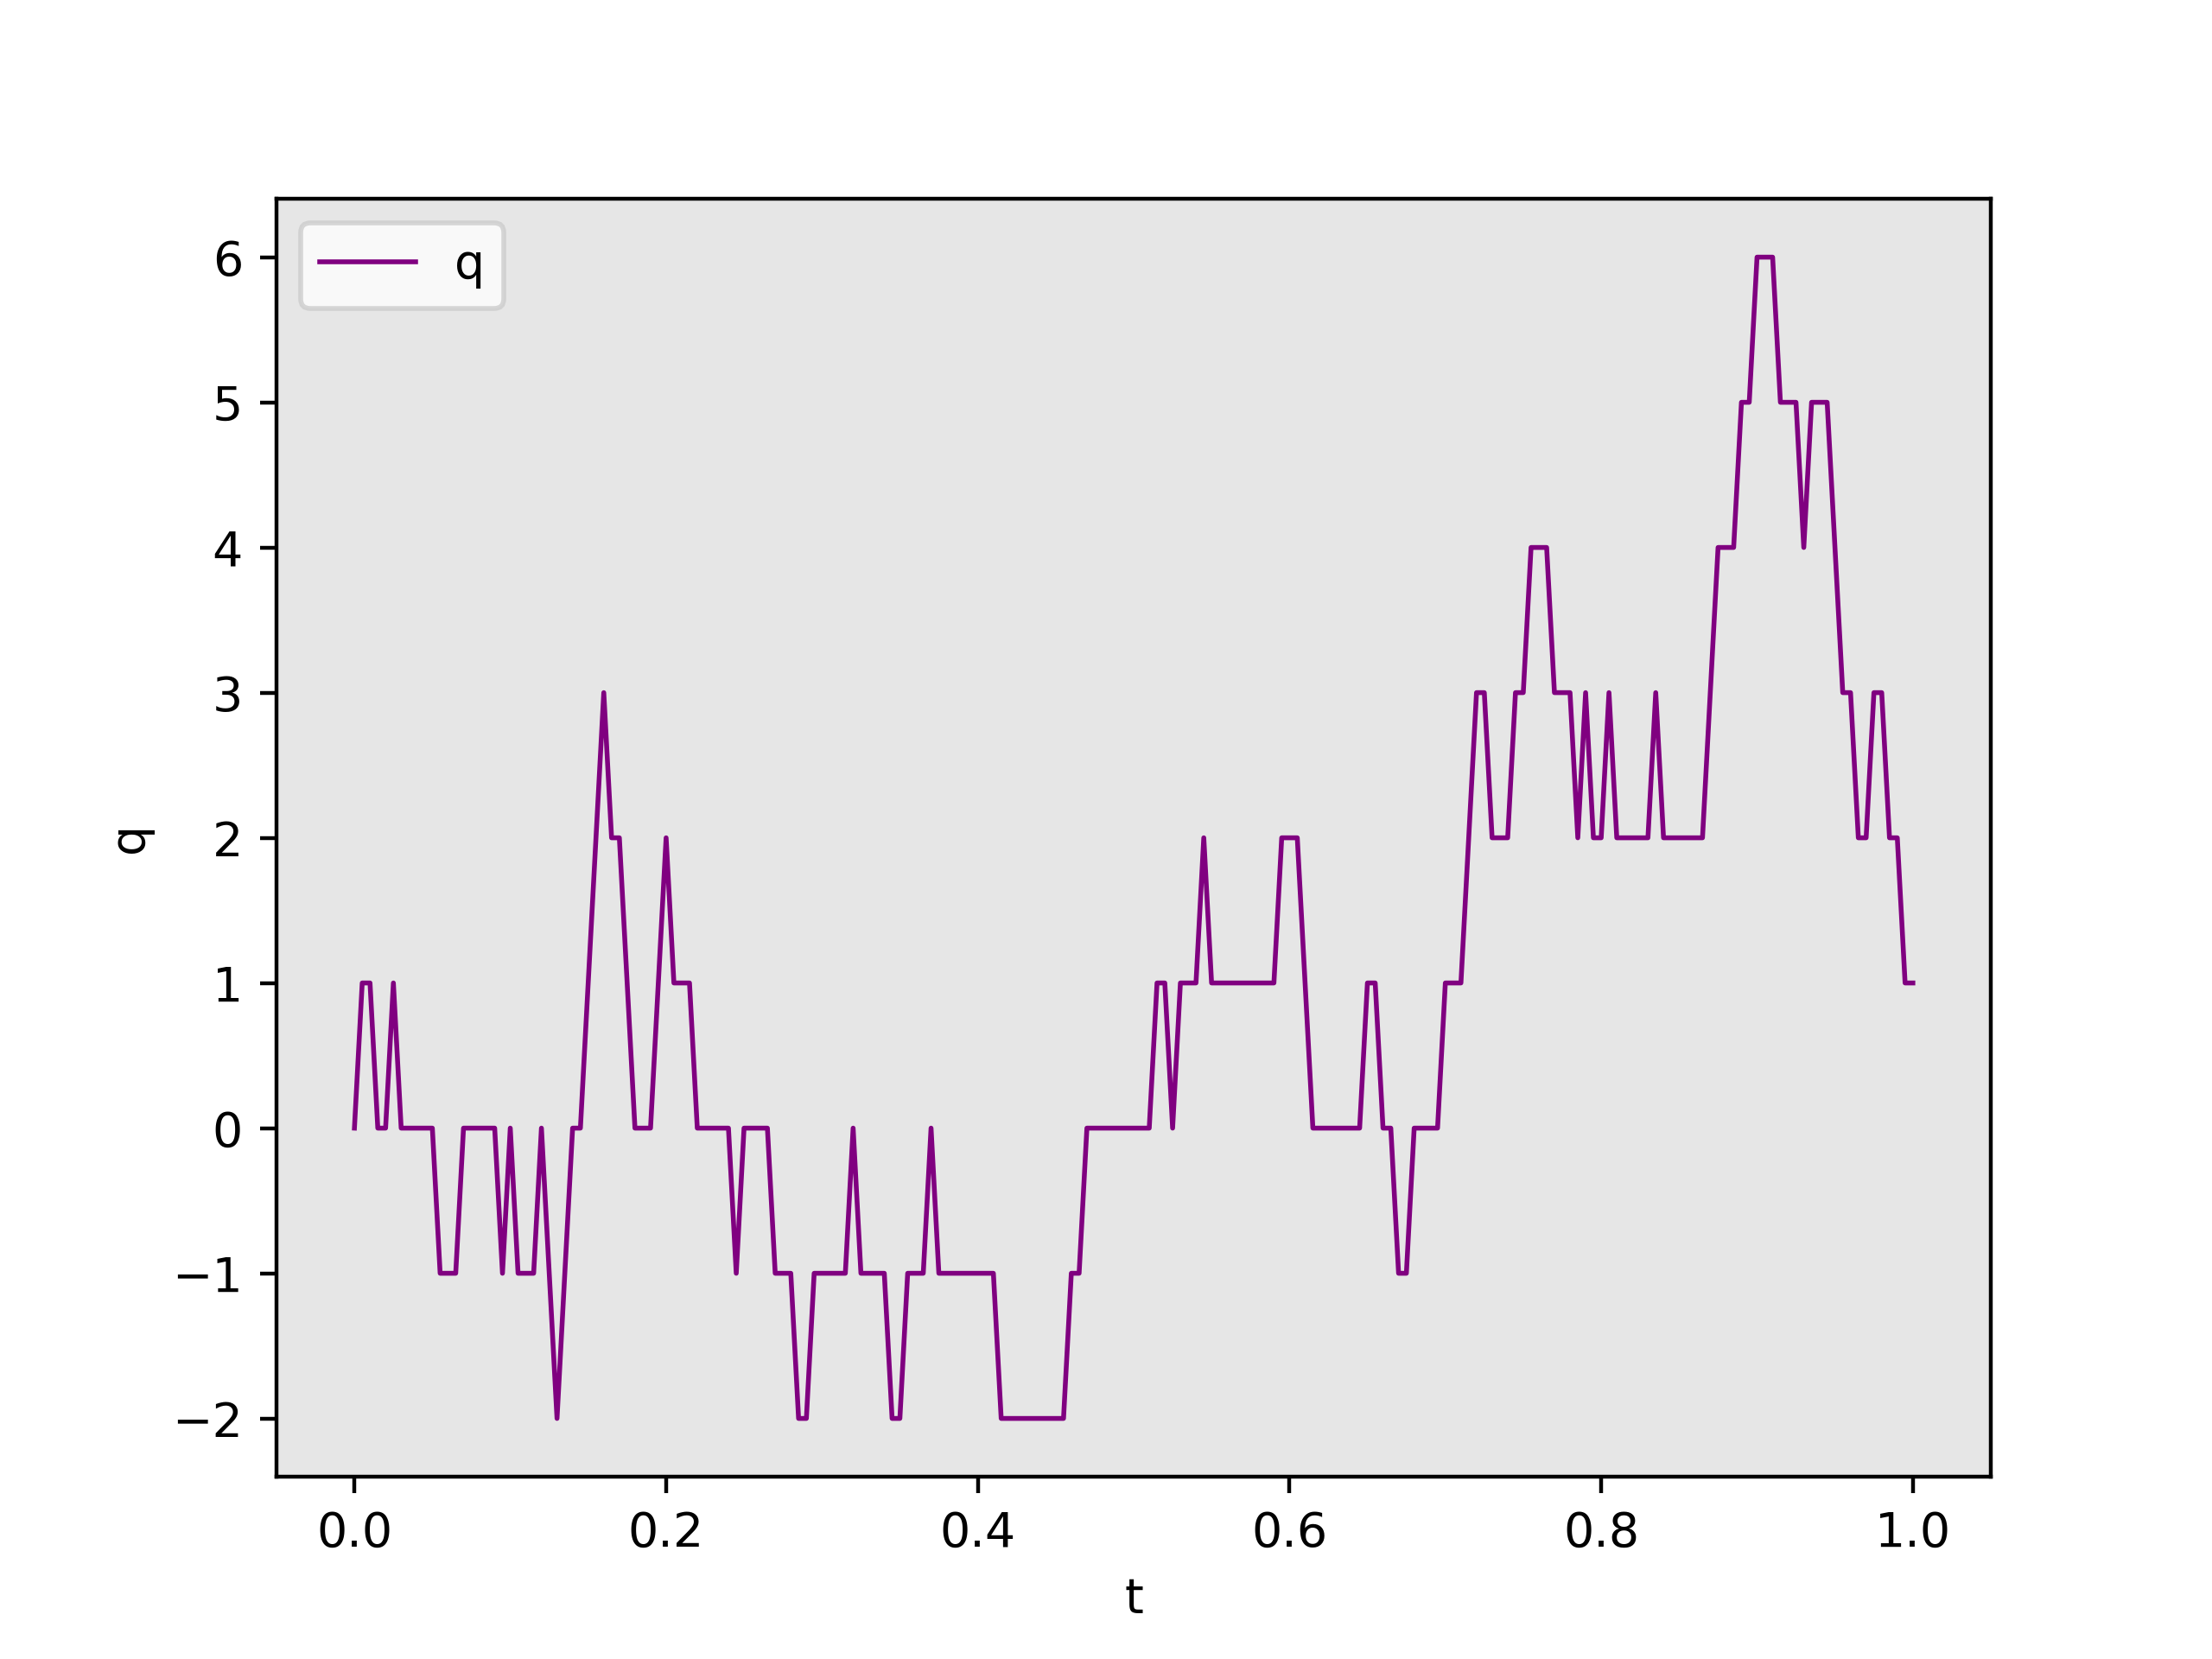
\includegraphics[scale=0.75]{inventory.png}
    \caption{Sample inventory for $\gamma=0.1$}
    \label{fig:inventory}
\end{figure}
\begin{figure}[ht!]
    \centering
    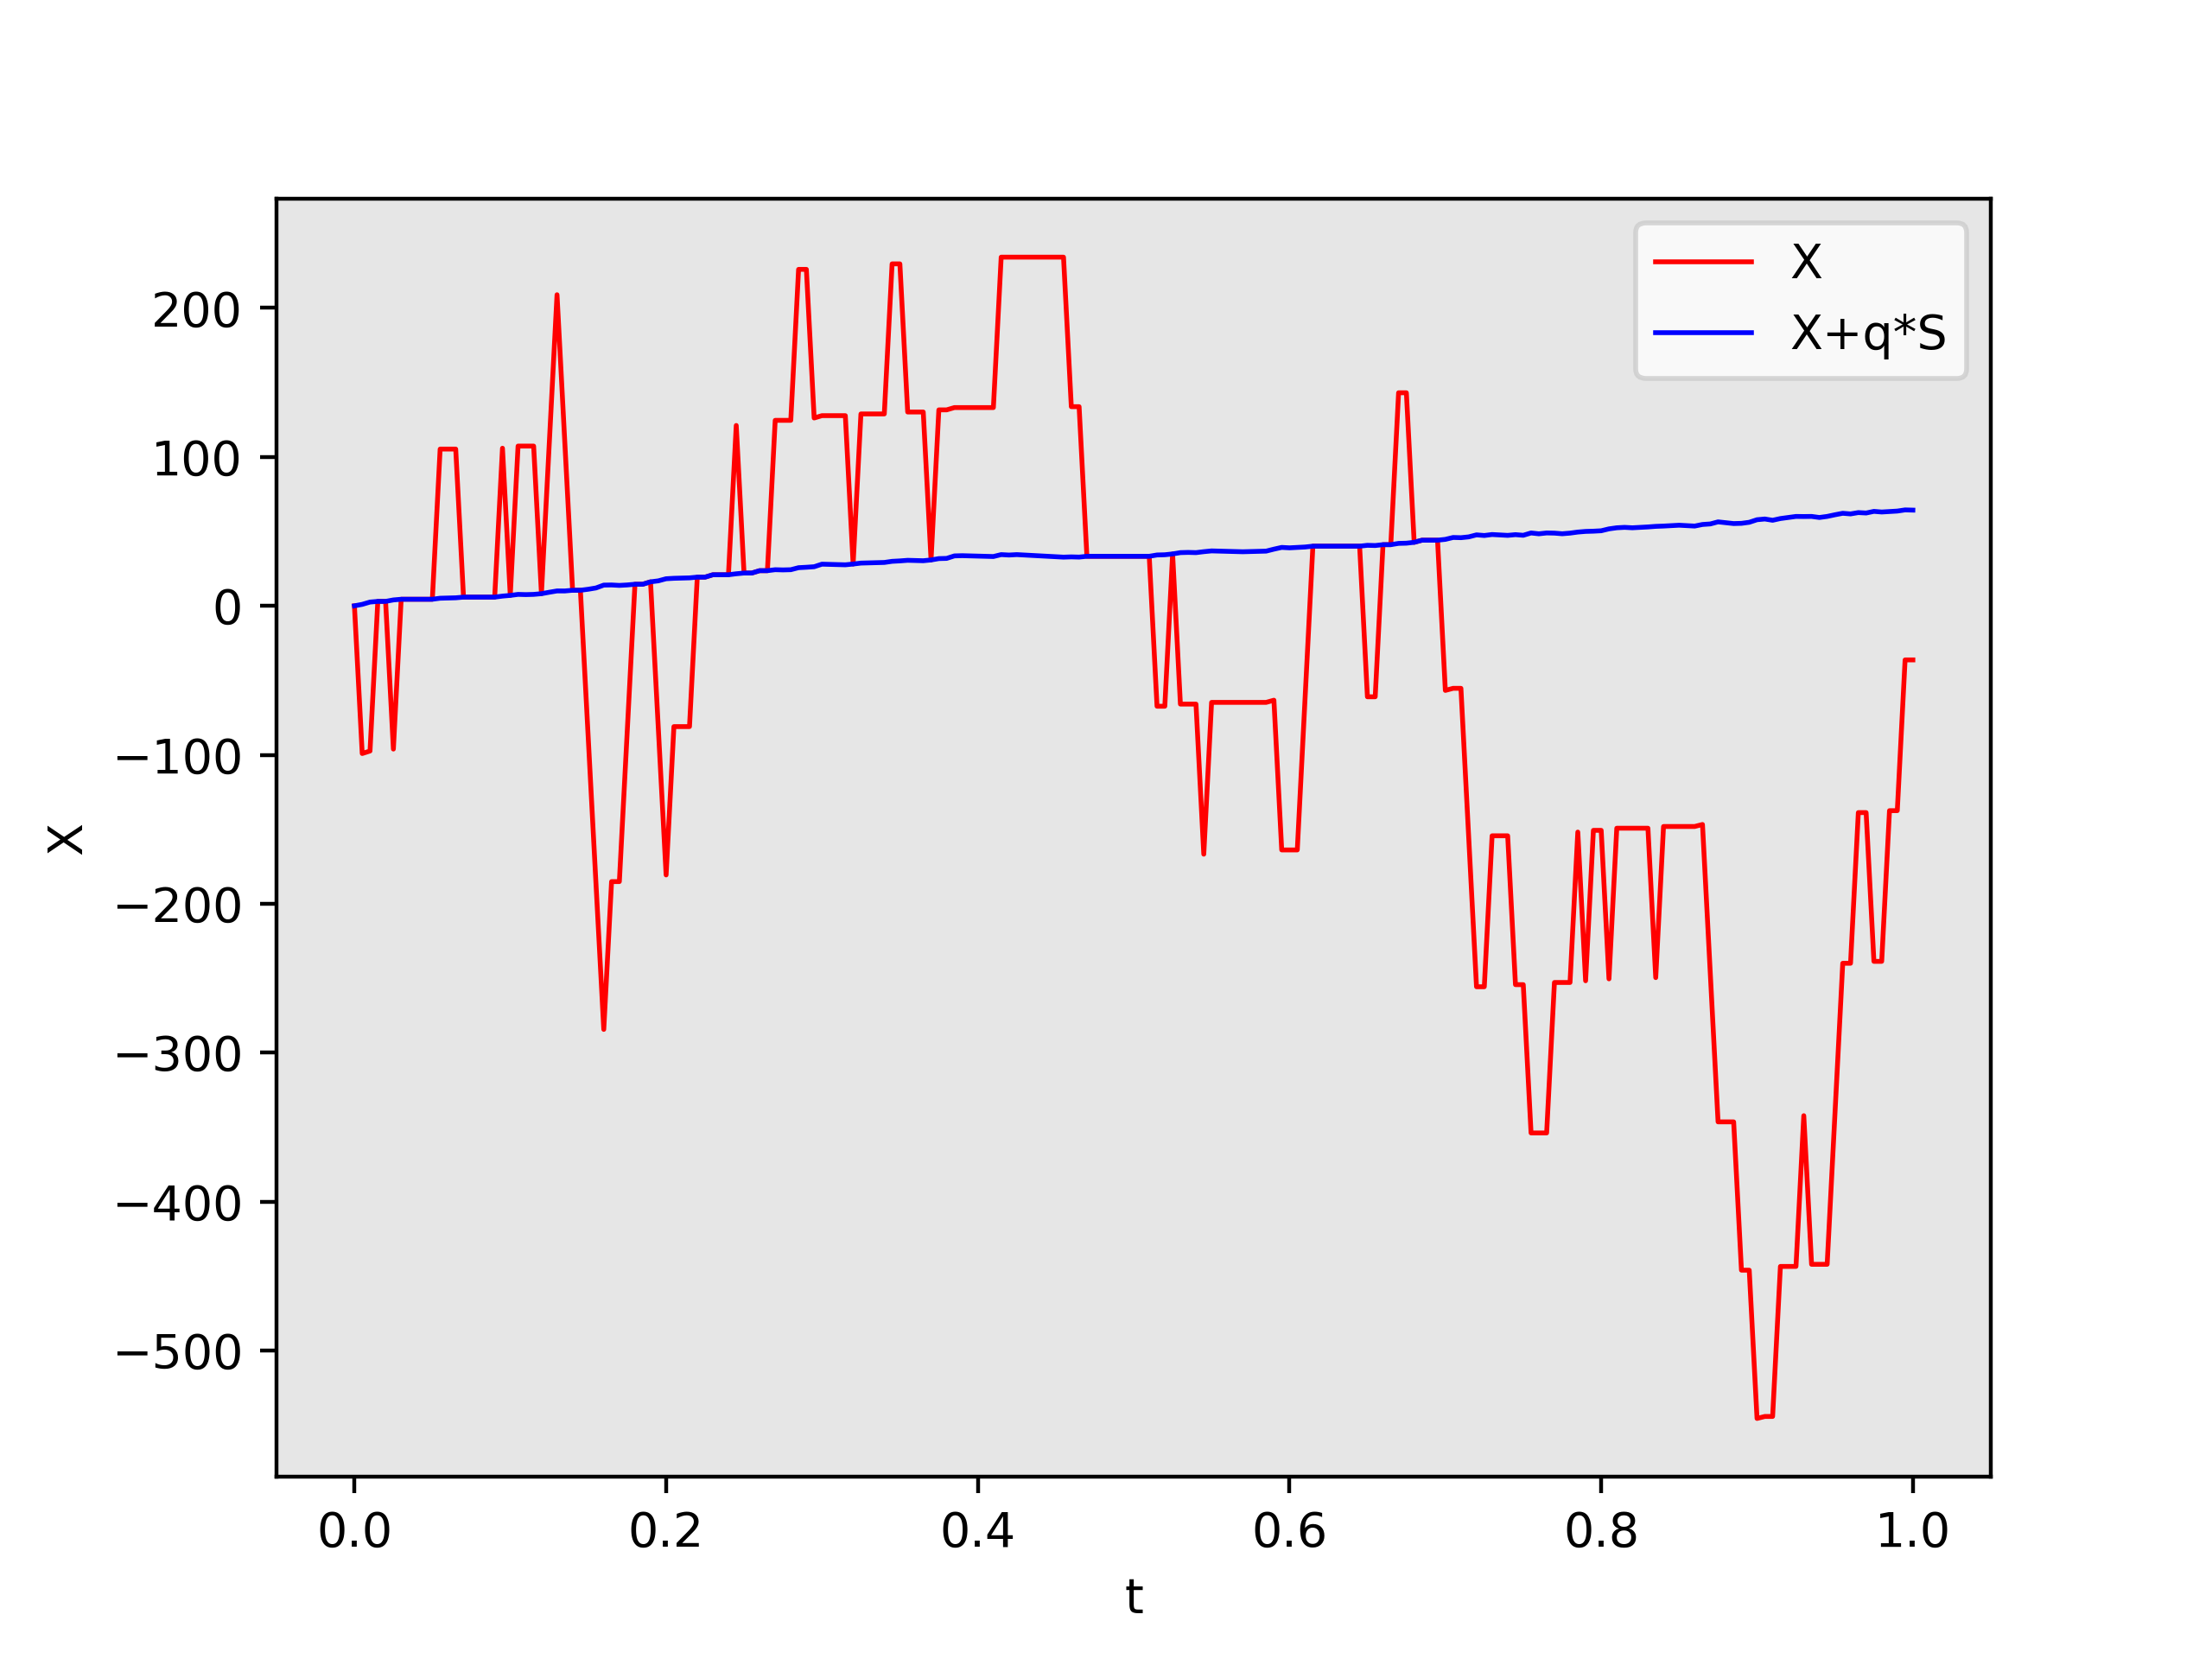
\includegraphics[scale=0.75]{wealth.png}
    \caption{Sample profit for $\gamma=0.1$}
    \label{fig:pnl}
\end{figure}

\begin{figure}[ht!]
    \centering
        \begin{tabular}{ c c c c c c } 
            \hline
            Strategy & $\mu$ (Spread) & $\mu$ (Profit) & $\sigma$ (Profit) & $\mu$ (Final q) & $\sigma$ (Final q) \\  
            \hline
            Inventory & 1.49 & 64.9 & 6.7 & 0.03 & 2.9 \\
            Symmetric & 1.49 & 68.2 & 13.1 & -0.1 & 8.3 \\
            \hline
        \end{tabular}
        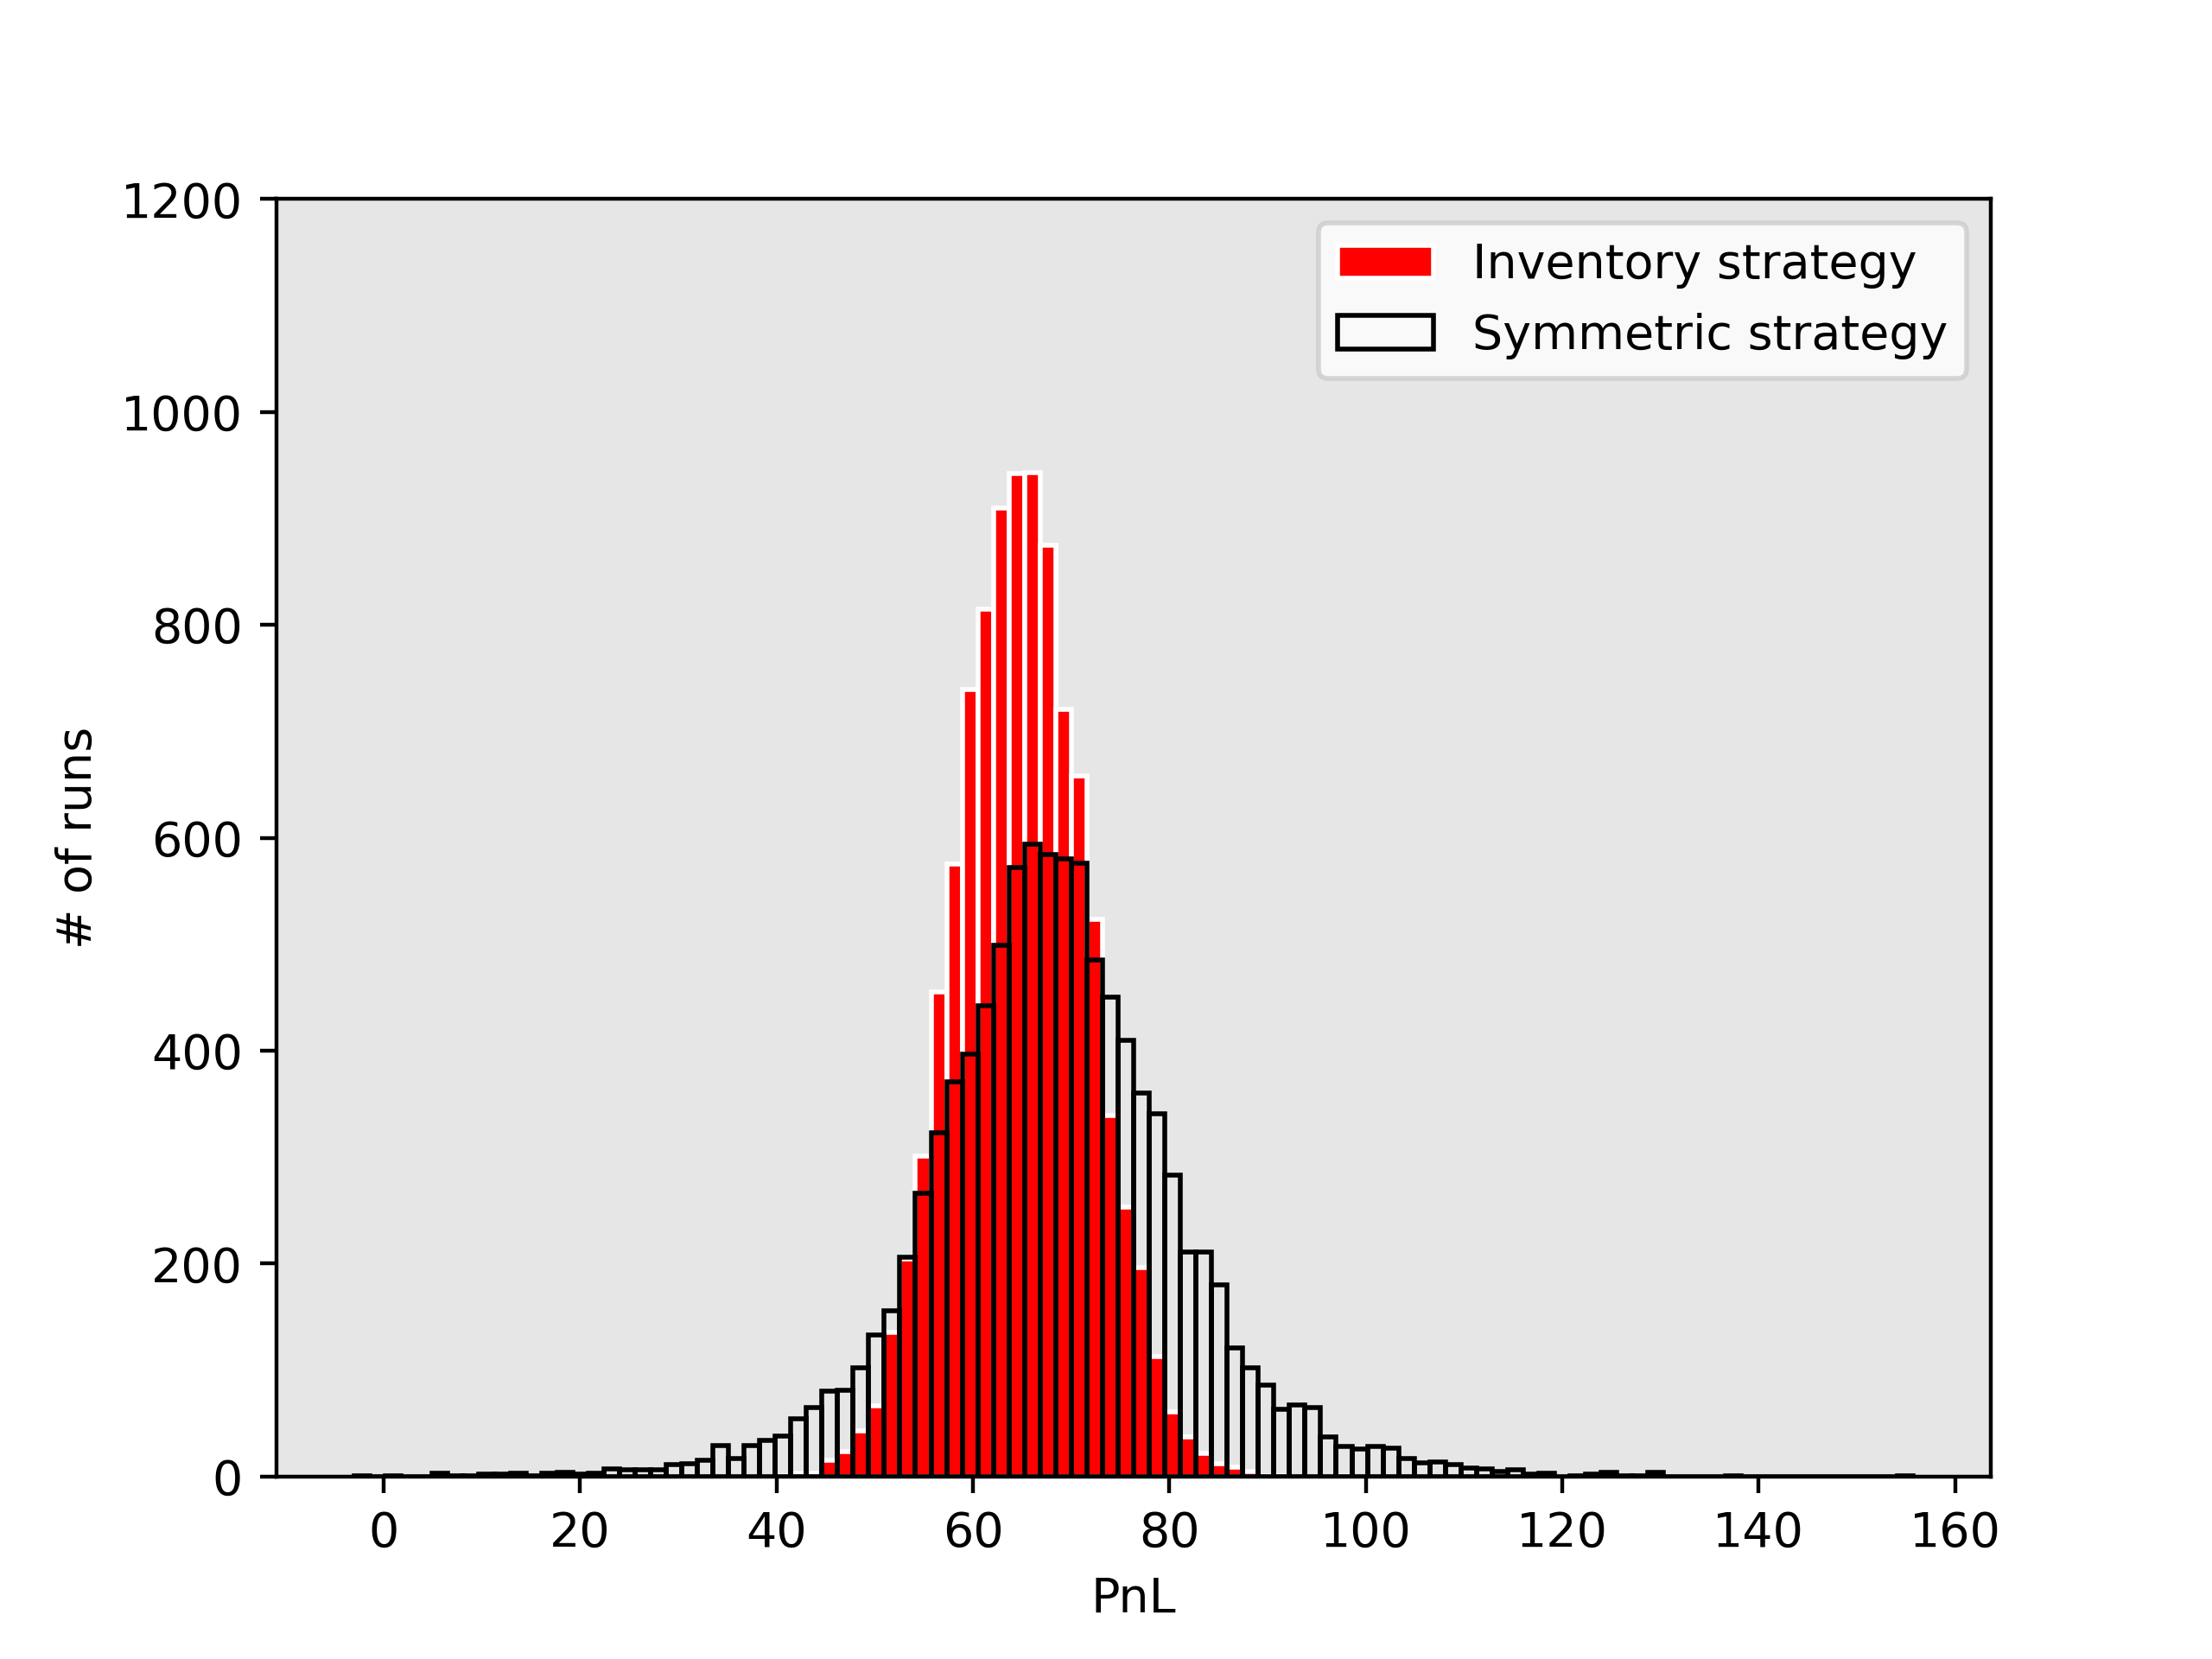
\includegraphics[scale=0.75]{gamma01.png}
        \caption{Results for $\gamma=0.1$}
        \label{fig:results-gamma01}
\end{figure}

In figure \ref{fig:results-gamma001} we present the results for 
10000 simulations with $\gamma=0.01$. Again, all of our figures 
closely match those presented by Avellaneda and Stoikov. In this case, we can see 
from the PnL distribution that there is less of a difference between the two strategies
now that we have a smaller $\gamma$, indeed, for $\gamma=0$ the agent is completely
inventory risk neutral and so the inventory strategy coincides with the symmetric 
strategy. It is interesting to note that in this case, the inventory and symmetric 
strategies achieve almost the same mean profit, but the standard deviation of the
inventory strategy is almost \$5 lower.

\begin{figure}
    \centering
        \begin{tabular}{ c c c c c c } 
            \hline
            Strategy & $\mu$ (Spread) & $\mu$ (Profit) & $\sigma$ (Profit) & $\mu$ (Final q) & $\sigma$ (Final q) \\ 
            \hline
            Inventory & 1.35 & 68.5 & 9.1 & 0.04 & 5.3 \\
            Symmetric & 1.35 & 68.6 & 13.8 & 0.04 & 8.6 \\
            \hline
        \end{tabular}
        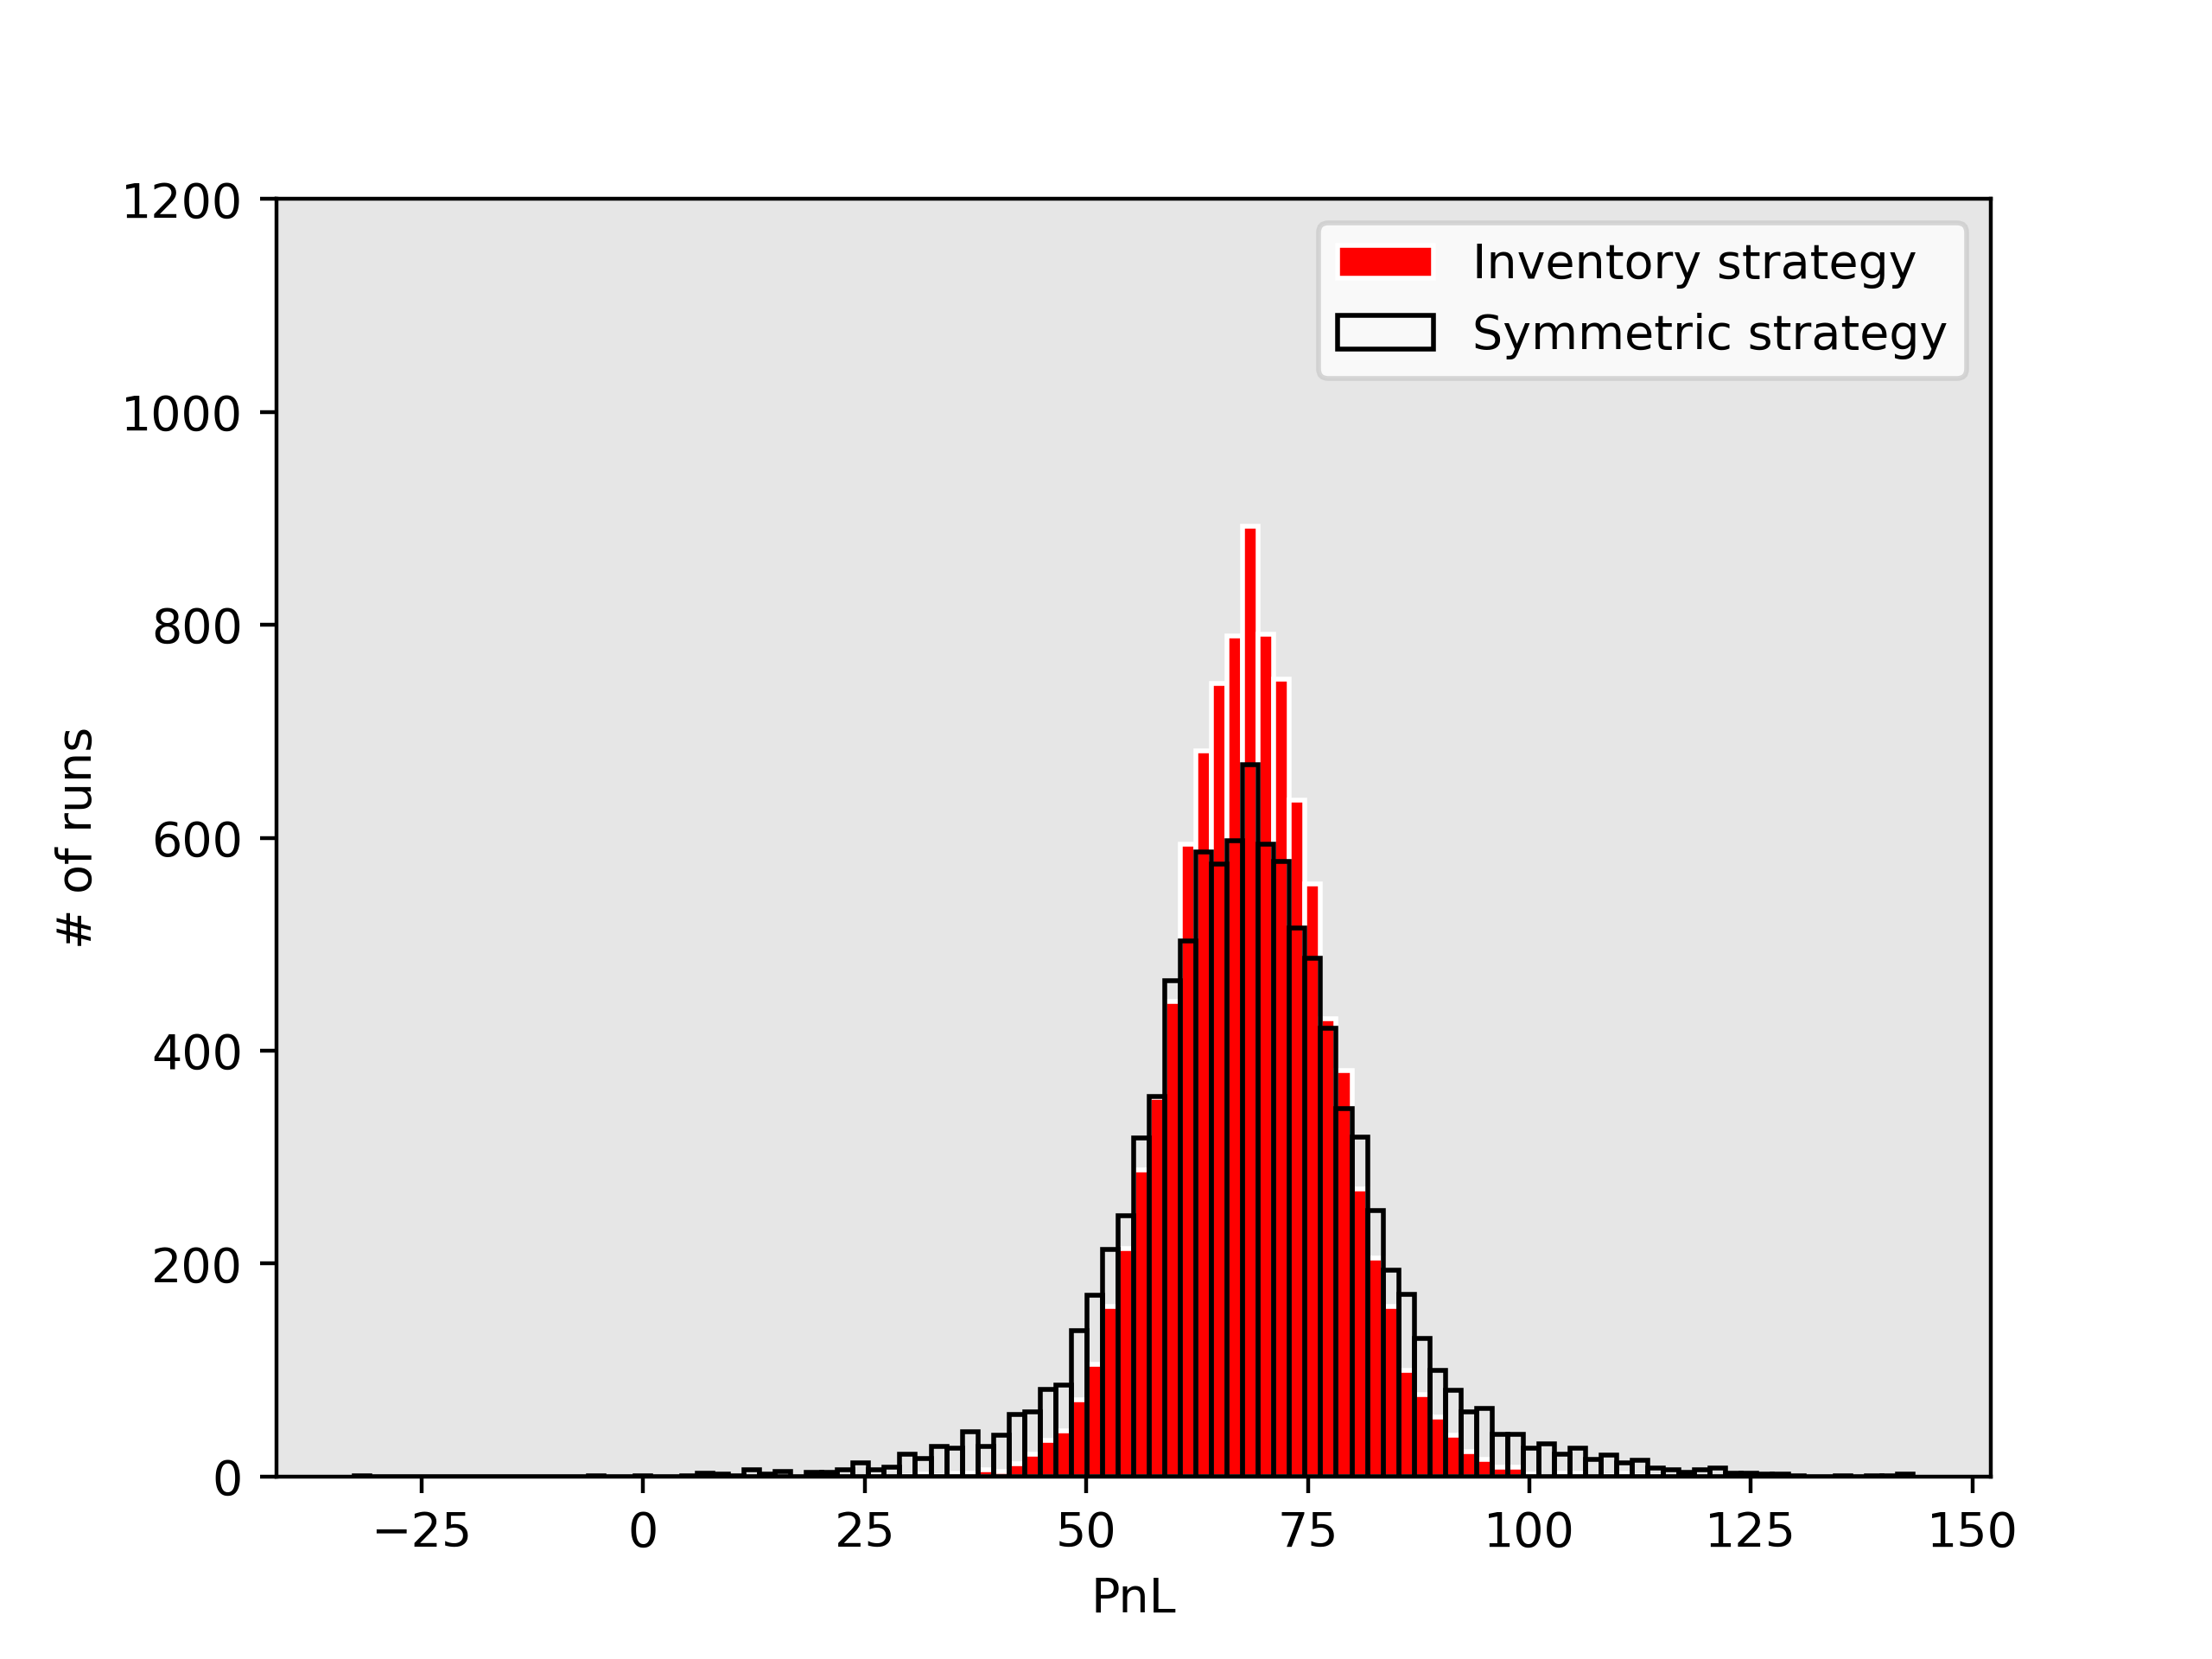
\includegraphics[scale=0.75]{gamma001.png}
        \caption{Results for $\gamma=0.01$}
        \label{fig:results-gamma001}
\end{figure}
